% !TEX encoding = UTF-8
% !TEX TS-program = pdflatex
% !TEX root = ../Tesi.tex
% !TEX spellcheck = en-EN

%************************************************
\chapter{Discrete Element Method}
\label{cap:dem}
%************************************************

The discrete element method (\acs{DEM}) is derived from Molecular Dynamics. \\ 
For each particle i inside the domain, a Discrete Element Method (\acs{DEM}) code
follows the trajectory and calculates the force that particle i exerts on particle j.
The main forces involved are: gravity, contact forces due to collisions, and
further interactions such as electrostatic, Van der Waals, cohesive forces and fluid-solid interactions in 
multiphase flows. \\
The two approaches can be implemented for this method are:
\begin{itemize}
  \item{hard spheres,}
  \item{soft spheres.}
\end{itemize} 
Thus, the hard-sphere approach is well-suited for binary collisions, easy to
calculate, but cannot predict multi-particle interactions.
It is mainly used for dilute flows, rather then in the dense flows we
investigated.

%\section{DEM}
%\label{sec:dem}
% \section{Hard spheres approach}
% \label{sec:hardspheresapproach}
% \info{words on hard spheres approach}

\section{Soft spheres approach}
\label{sec:softspheresapproach}

\begin{figure}[!h]
\centering
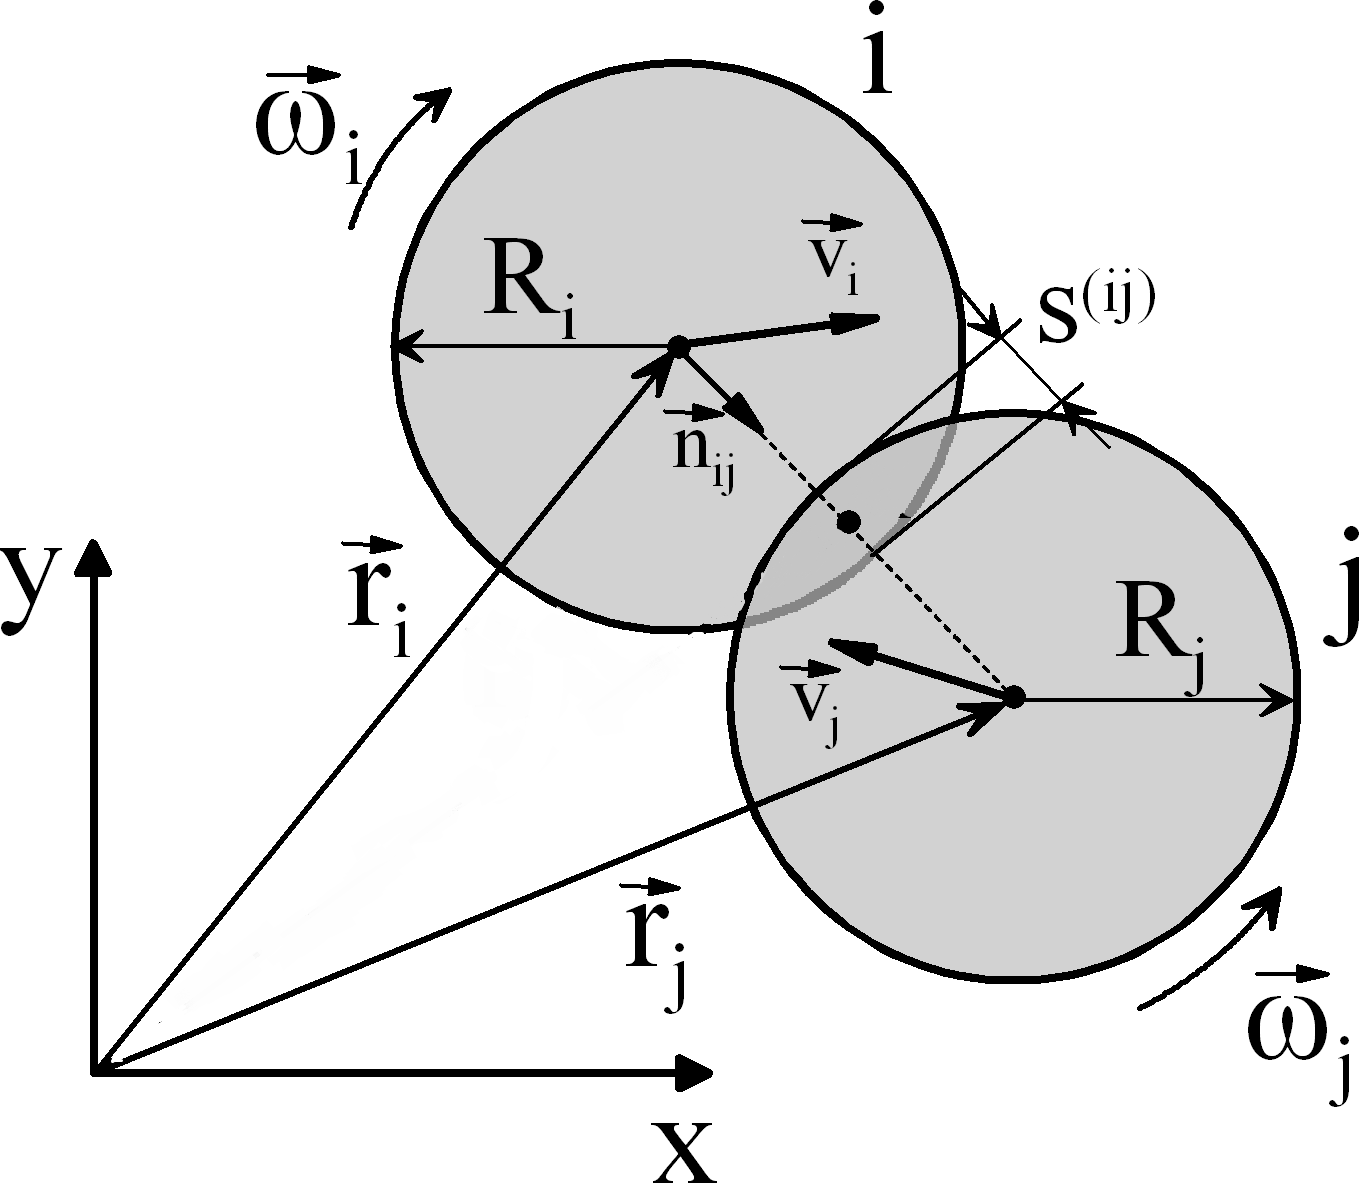
\includegraphics[width=.6\columnwidth]{images/109twospheres}
\caption[Two spheres]{Two colliding spheres with the soft-sphere approach.}
\label{fig:109twospheres}
\end{figure}
The soft-sphere approach consider the deformations of the particles when they
collide with each other. From the vector in Fig. \ref{fig:109twospheres} we can
define after time \textit{t} the normal and tangential overlaps \acs{xin} and
\acs{xit}:
\begin{equation}
\xi_n = R_i + R_j - \mathbf{n} \cdot (\mathbf{r}_j - \mathbf{r}_i),
 \label{eq:xin}
\end{equation}

\begin{equation}
\xi_t = \int_{0}^{t}{\mathit{dt'}|\mathbf{v}_t(\mathit{t'})|} ,
 \label{eq:xit}
\end{equation}

For an elasto-perfectly-plastic-viscous model the contact forces, normal and
tangential, are:
\begin{equation}
\mathbf{F}_{n} = k_n \xi_n \mathbf{n} + \gamma_n \mathbf{v}_n , 
\label{eq:fn}
\end{equation}

\begin{equation}
\mathbf{F}_t = 
 \begin{cases}
k_t \xi_t \mathbf{t} + C_t \mathbf{v}_t  & \text{if } |k_t \xi_t \mathbf{t} +
C_t \mathbf{v}_t| \leq \mu_s |\mathbf{F}_n| ,\\
\mathbf{t} \mu_s |\mathbf{F}_n|  & \text{else.}
\end{cases}
 \label{eq:ft}
\end{equation}
%************************************************
The Coulomb's law of friction is the condition in the tangential force
formulation.
At this point we can divide the contact models into:
\begin{itemize}
  \item{linear, e.g. Hooke,}
  \item{non-linear, e.g. Hertz.}
\end{itemize}

\improvement{introduce the rolling friction}
Rolling friction:
\begin{itemize}
  \item{cdt;}
  \item{epsd;}
  \item{epsd2.}
\end{itemize}

% \subsection{Hooke}
% \label{subsec:hooke}

\subsection{Hertz}
\label{subsec:hertz}

For the raw material used in this work 
Di Renzo and Di Maio \cite{RefWorks:145} suggested using the non-linear
Hertzian model without cohesion for the particle-particle and particle-wall contacts. 
This granular model uses the following formula for the contact force between two granular particles (Eq. \ref{eq:forceij}):
%************************************************
\begin{equation}
 F_{ij} = 
\begin{cases}
F_{n,ij} + F_{t,ij} = \left( k_n \delta_{n,ij} + \gamma_n v_{n,ij} \right) + \left( k_t \delta_{t,ij} + \gamma_t v_{t,ij} \right) & \text{if } r < d ,\\
0    & \text{if } r > d ,\\
\end{cases}
 \label{eq:forceij}
\end{equation}

%************************************************
where the subscript \acs{n} stands for normal and \acs{t} for tangential. 
Here, $k$ and $\gamma$ are respectively the stiffness and damping coefficients, 
while $\delta$ and $v$ are the displacement and the velocity, $r$ is the
distance between two particles of radii $R_i$ and $R_j$, and $d = R_i + R_j $ is
the contact distance.
Both the normal and the tangential
force comprise two terms, a spring force and a damping force. 
The tangential (or shear) force is a ``history'' effect that accounts for the
tangential displacement (``tangential overlap'') between the particles for the
duration of contact.
The $k_n$, $k_t$, $\gamma_n$, and $\gamma_t$ coefficients are calculated from
the material properties as follows:
%************************************************
\begin{equation}
\begin{aligned}
	k_n &= \frac{4}{3} E_{eq} \sqrt{R_{eq} \xi_n} ,\\
	\gamma_n &= 2 \sqrt{\frac{5}{6}} \beta \sqrt{S_n m_{eq}} ,\\
	k_t &= 8 G_{eq} \sqrt{R_{eq}} \xi_n ,\\
	\gamma_t &= 2 \sqrt{\frac{5}{6}} \beta \sqrt{S_t m_{eq}} .
\end{aligned}
\label{eq:hertz}
\end{equation}

%************************************************
In addition to the equations \ref{eq:hertz} the following relations (Eqns. \ref{eq:equivProp2}) are required:
%************************************************
\begin{equation}
\begin{aligned}
 \frac{1}{E_{eq}} & = \frac{1-\nu_i^2}{E_i} + \frac{1-\nu_j^2}{E_j} ,\\
 \frac{1}{G_{eq}} & = \frac{2(2+\nu_i)(1-\nu_i)}{E_i} + \frac{2(2+\nu_j)(1-\nu_j)}{E_j} ,\\
 \frac{1}{R_{eq}} &= \frac{1}{R_i} + \frac{1}{R_j} ,\\
 \frac{1}{m_{eq}} &= \frac{1}{m_i} + \frac{1}{m_j} ,\\
 \beta & = \frac{\ln(e)}{\sqrt{ln^2(e)+\pi^2}} ,\\
 S_n & = 2 E_{eq} \sqrt{R_{eq} \delta_n} ,\\
 S_t & = 8 G_{eq} \sqrt{R_{eq} \delta_n} ,\\
 k_r & = k_t R_{eq}^2 .\\
\end{aligned}
\label{eq:equivProp2}
\end{equation}


%************************************************

In the paper by Wensrich and Katterfeld \cite{RefWorks:87}, further details on
the method can be found.\\
In the contact law we used, 
the tangential component of the contact force between two generic particles
($F_t$) is truncated to fulfil:
%************************************************
\begin{equation}
F_{t,ij} \leq \mu_s F_{n,ij},
 \label{eq:force_t}
\end{equation}

%************************************************

where $F_n$ is the normal component and \acs{mus} is the coefficient of sliding
friction, one of the particle-based \acs{DEM} parameter we investigated, 
another being the coefficient of rolling friction (\acs{mur}). 

\subsection{EPSD2}
\label{subsec:epsd2}

For coarse non-spherical particles, this is a critical parameter and describes
inter-particle friction in medium to dense granular flow simulations. It is proportional to the 
torque counteracting the rotation of the particle. The \acs{mur} parameter enters the 
equations according to the elasto-rolling resistance model presented by Wensrich and 
Katterfeld \cite{RefWorks:87} and Ai et al. \cite{RefWorks:131} 
based on the work of Jiang et al. \cite{RefWorks:143}. 
The model is called $EPSD2$ in \acs{LIGGGHTS} and is appropriate for both one-way and cyclical rolling cases.
The maximum magnitude of rolling resistance torque is (Eq. \ref{eq:trmax}):

%************************************************
\begin{equation}
T_{r~max} = \mu_r R_r |\tilde{F_n}| ~,
 \label{eq:trmax}
\end{equation}

%************************************************

where $R_r$ is the equivalent radius and $F_n$ the normal force.
The last two particle-based \acs{DEM} parameters we investigated were \acs{rhop}
and the coefficient of restitution (\acs{CoR}) as defined by Ai. et al.
\cite{RefWorks:131}.
Together with the others they are listed in Table \ref{tab:08DEMparameters}.\\

\begin{table}[h]
\centering
\begin{tabular}{l}
\hline 
    Radius \ac{R} (m)   \\ [5pt]

	Size distribution (-) \\ [5pt]

    Young's modulus \ac{E} (Pa)  \\ [5pt]

    Poisson's ratio \ac{nu} (-) \\ 
     Time step \ac{deltat} (s) \\ [5pt]
        \hline
     Coefficient of sliding friction \ac{mus} (-)\\  [5pt]
    Coefficient of rolling friction \ac{mur} (-) \\ [5pt]
    Coefficient of restitution \ac{CoR} (-)   \\ [5pt]
     Particle density $\ac{rhop} = \frac{mass ~ of ~ one ~ particle}{volume ~ of
     ~ one ~ particle}$ ($kg/m^3$)  \\ [5pt]
     Geometry factor \ac{dCylDp} (-)  \\ [5pt]
   
\hline
\end{tabular}
\caption[DEM parameters]{DEM parameters. The upper parameters were
identical in all simulations. The lower parameters were constant in each
simulation, but were varied between simulations.}
\label{tab:08DEMparameters}
\end{table}



\section{Literature Values}
\label{sec:literaturevalues}

\improvement{Discuss about literature values for all parameters (ref.
Combarros, Paulick).}